\chapter{History}
\label{sec:history}

ngscopeclient saves a rolling buffer of previous waveforms in memory, allowing you to go back in time and see previous
state of the system being debugged. This buffer is included in saved sessions, allowing a full snapshot of system
behavior to be loaded for future analysis. History is always captured up to the configured depth, regardless of whether
the history view window is displayed or not.

Clicking on a timestamp in the history view (Fig. \ref{historyview}) pauses acquisition and loads the historical
waveform data for analysis.

\begin{figure}[H]
\centering
\includegraphics[width=7cm]{ng-images/history.png}
\caption{Waveform history view}
\label{historyview}
\end{figure}

Hovering the mouse over a row in the history view (Fig. \ref{history-tooltip}) displays a tooltip with the full date
and time of the acquisition, as well as some information about which instruments and channels had data in the capture
(if some channels were enabled or disabled during the lab session, the set of active channels may have changed
throughout history).

\begin{figure}[H]
\centering
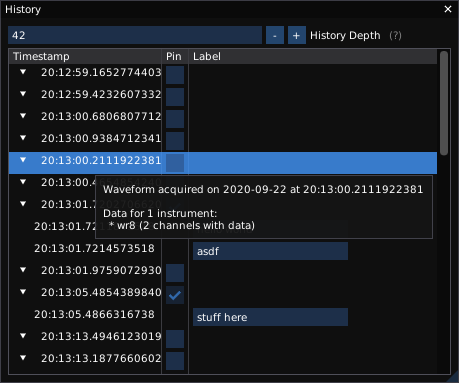
\includegraphics[width=7cm]{ng-images/history-tooltip.png}
\caption{Tooltip on waveform history entry}
\label{history-tooltip}
\end{figure}

The history depth defaults to 10 waveforms, but can be set arbitrarily within the limits of available RAM. All history
must fit in system RAM in the current software version; spilling to disk is planned for the future
(\issue{scopehal-apps}{311}). Older waveforms beyond the history limit are deleted automatically as new waveforms are
acquired. Any single waveform in history may also be deleted by right clicking on the line and selecting ``delete" from
the menu.

%The status bar at the bottom of the history view displays the total number of waveforms in the history, as well as an
%estimate of the amount of RAM used by the history.

\section{Pinning}

Interesting waveforms may be ``pinned" in the history by checking the box in the ``pin" column of the history view.
Pinned waveforms are retained in the history buffer even when new waveforms arrive; only unpinned waveforms
are eligible for automatic deletion to make space for incoming data.

If a waveform contains markers (\ref{sec:markers}), it is automatically pinned and cannot be unpinned unless the marker
(or entire waveform) is manually deleted. This prevents accidental loss of an important waveform: if the event was
important enough to mark and name, it is probably worth keeping around.

\section{Labeling}

Arbitrary text names may be assigned to a waveform by clicking the corresponding cell in the ``label" column. As with
waveforms containing markers, waveforms with a label are automatically pinned since assigning a label implies the
waveform is important.

\begin{comment}

\section{Estimating Waveform Memory Usage}

When selecting a maximum depth for the history, it is important to pick a reasonable limit to avoid running out of RAM!
ngscopeclient will happily fill tens or hundreds of gigabytes of memory with deep waveforms if given a chance. Memory
usage of waveform data can be roughly estimated as 16 + sizeof(sample type) bytes per point, since each sample contains a
64-bit timestamp and duration plus the sample data.

For example, an analog sample takes 20 bytes of RAM (16 of time plus a 32-bit floating point voltage measurement) per
sample. Thus, a 1M point analog waveform takes approximately 20 MB of RAM per channel, or 80 MB per capture on a
four-channel oscilloscope with all channels enabled.

On the larger side, a 10M point four channel capture would use 800 MB and a 64M point deep-memory capture would use 5
GB. A deep history setting, such as 100 waveforms, is thus wildly inappropriate for such deep captures! A future
software release may support spilling waveform data to a temporary directory on disk, permitting effectively unlimited
history depth given sufficient disk space.

Digital waveforms use one byte per sample for the actual measurement, so 17 MB per channel for a 1M point waveform.
Most logic analyzer or MSO drivers for libscopehal will perform automatic de-duplication when a waveform goes several
clock cycles with no toggles, so the actual memory usage is likely to be significantly less than this.

Filter memory usage varies depending on the specific filter in question, however it is typically not a large
contributor to the overall ngscopeclient RAM footprint when using history mode because filters are evaluated
dynamically each time a waveform is pulled from history rather than having output cached for every historical waveform.
Thus, at most one copy of each filter's output is present in memory regardless of history depth.
\end{comment}
